\documentclass{article}
\usepackage{amsmath, sfmath, multicol, tkz-euclide, array, enumerate, tcolorbox, tabularray}
\renewcommand{\familydefault}{\sfdefault}
\setlength{\parindent}{0cm}
\pagestyle{empty}
\usepackage[left=1in, top=0.5in, right=1in, bottom=0.5in]{geometry}
\tikzset{>=stealth}
\tcbset{colback=white}

\newcounter{example}[section]
\newenvironment{example}[1][]{\refstepcounter{example}\par\medskip
   {\color{red}\textbf{Example~\theexample. #1}}}{\medskip}

\begin{document}

\section*{Proving Triangles Similar}

\begin{tcolorbox}[colframe=orange!70!white, coltitle=black, title=\textbf{Today I Can}]
\begin{enumerate}
    \item Use the AA Similarity Postulate and the SAS and SSS Similarity Theorems.
\end{enumerate}
\end{tcolorbox}
\smallskip

\begin{tcolorbox}[colframe=black!20!white, opacitybacktitle=0.1, coltitle=black, title=\textbf{Angle-Angle (AA) Similarity}]
If two angles of one triangle are congruent to two angles of another, then the triangles are similar. \newline 

\begin{minipage}{0.55\textwidth}
\begin{itemize}
    \item $\angle A \cong \angle D \text{ and } \angle C \cong \angle F \implies \triangle ABC \sim \triangle DEF$
\end{itemize}
\end{minipage}
\begin{minipage}{0.4\textwidth}
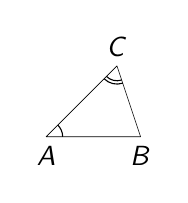
\begin{tikzpicture}[scale=0.6]
\tkzDefPoints{0/0/A, 2/0/B, 1.5/1.5/C}
\tkzDrawPolygon(A,B,C)
\tkzMarkAngle[size=0.35](B,A,C)
\tkzMarkAngle[arc=ll, size=0.35](A,C,B)
\tkzLabelPoints[below](A,B)
\tkzLabelPoints[above](C)
\end{tikzpicture}
\hspace{0.25in}
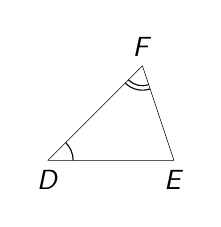
\begin{tikzpicture}[scale=0.8]
\tkzDefPoints{0/0/D, 2/0/E, 1.5/1.5/F}
\tkzDrawPolygon(D,E,F)
\tkzMarkAngle[size=0.4](E,D,F)
\tkzMarkAngle[arc=ll, size=0.35](D,F,E)
\tkzLabelPoints[below](D,E)
\tkzLabelPoints[above](F)
\end{tikzpicture}
\end{minipage}
\end{tcolorbox}

\begin{example}
Are the 2 triangles similar? How do you know?
\begin{multicols}{2}
\begin{enumerate}[(a)]
    \item $\triangle RSW$ and $\triangle VSB$
    \item $\triangle JKL \text{ and } \triangle PQR$
\end{enumerate}
\end{multicols}
\begin{minipage}{0.45\textwidth}
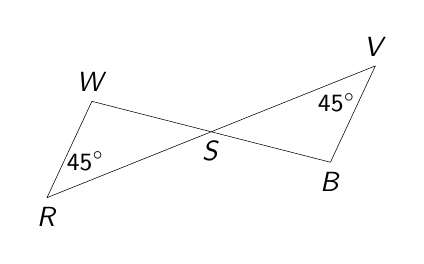
\begin{tikzpicture}[scale=0.9]
\tkzDefPoints{0/0/R, 4/0.5/B}
\tkzDefShiftPoint[R](65:1.5){W}
\tkzDefShiftPoint[B](65:1.5){V}
\tkzDrawPolygon(R,W,B,V)
\tkzInterLL(R,V)(B,W)
\tkzGetPoint{S}
\tkzLabelPoints[below](R,S,B)
\tkzLabelPoints[above](W,V)
\tkzLabelAngle[pos=0.75](V,R,W){\small $45^\circ$}
\tkzLabelAngle[pos=0.75](S,V,B){\small $45^\circ$}
\end{tikzpicture}
\end{minipage}
\begin{minipage}{0.45\textwidth}
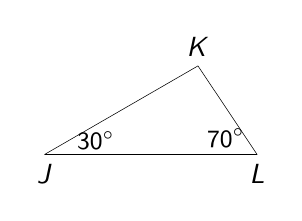
\begin{tikzpicture}[scale=0.9]
\tkzDefPoints{0/0/J, 3/0/L}
\tkzDefShiftPoint[J](30:2.5){K}
\tkzDrawPolygon(J,K,L)
\tkzLabelPoints[below](J,L)
\tkzLabelPoints[above](K)
\tkzLabelAngle[pos=0.75](L,J,K){\small $30^\circ$}
\tkzLabelAngle[pos=0.5](K,L,J){\small $70^\circ$}
\end{tikzpicture}
\hspace{0.1in}
\begin{tikzpicture}[scale=0.9]
\tkzDefPoints{0/0/P, -3/0/R}
\tkzDefShiftPoint[J](150:2.5){Q}
\tkzDrawPolygon(P,Q,R)
\tkzLabelPoints[below](P,R)
\tkzLabelPoints[above](Q)
\tkzLabelAngle[pos=0.4](R,Q,P){\small $85^\circ$}
\tkzLabelAngle[pos=0.65](P,R,Q){\small $70^\circ$}
\end{tikzpicture}
\end{minipage}
\end{example}

\vfill 

\begin{tcolorbox}[colframe=black!20!white, opacitybacktitle=0.1, coltitle=black, title=\textbf{Side-Angle-Side (SAS) Similarity}]
If two pairs of sides of one triangle are proportional to two pairs of sides of another and the included angles are congruent, then the triangles are similar.\newline 

\begin{minipage}{0.55\textwidth}
\begin{itemize}
    \item If $\frac{AB}{DE} = \frac{AC}{DF}$
    \item and $\angle A \cong \angle D$
    \item then $\triangle ABC \sim \triangle DEF$
\end{itemize}
\end{minipage}
\begin{minipage}{0.4\textwidth}
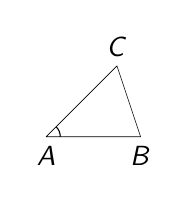
\begin{tikzpicture}[scale=0.6]
\tkzDefPoints{0/0/A, 2/0/B, 1.5/1.5/C}
\tkzDrawPolygon(A,B,C)
\tkzMarkAngle[size=0.3](B,A,C)
\tkzLabelPoints[below](A,B)
\tkzLabelPoints[above](C)
\end{tikzpicture}
\hspace{0.25in}
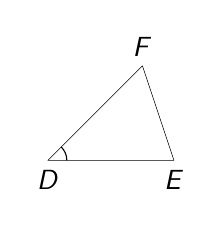
\begin{tikzpicture}[scale=0.8]
\tkzDefPoints{0/0/D, 2/0/E, 1.5/1.5/F}
\tkzDrawPolygon(D,E,F)
\tkzMarkAngle[size=0.3](E,D,F)
\tkzLabelPoints[below](D,E)
\tkzLabelPoints[above](F)
\end{tikzpicture}
\end{minipage}
\end{tcolorbox}

\begin{tcolorbox}[colframe=black!20!white, opacitybacktitle=0.1, coltitle=black, title=\textbf{Side-Side-Side (SSS) Similarity}]
If the lengths of the 3 sides of one triangle are proportional to the lengths of another, then the triangles are similar.\newline 

\begin{minipage}{0.55\textwidth}
\begin{itemize}
    \item $\dfrac{AB}{DE} = \dfrac{BC}{EF} = \dfrac{AC}{DF} \implies \triangle ABC \sim \triangle DEF$
\end{itemize}
\end{minipage}
\begin{minipage}{0.4\textwidth}
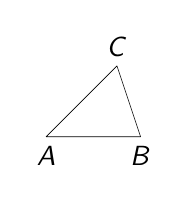
\begin{tikzpicture}[scale=0.6]
\tkzDefPoints{0/0/A, 2/0/B, 1.5/1.5/C}
\tkzDrawPolygon(A,B,C)
\tkzLabelPoints[below](A,B)
\tkzLabelPoints[above](C)
\end{tikzpicture}
\hspace{0.25in}
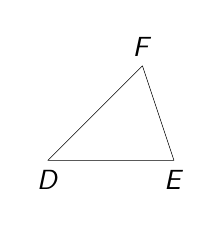
\begin{tikzpicture}[scale=0.8]
\tkzDefPoints{0/0/D, 2/0/E, 1.5/1.5/F}
\tkzDrawPolygon(D,E,F)
\tkzLabelPoints[below](D,E)
\tkzLabelPoints[above](F)
\end{tikzpicture}
\end{minipage}
\end{tcolorbox}

\newpage 

\begin{example}
Determine if the two triangles are similar in each. If so, write a similarity statement.
\begin{multicols}{2}
\begin{enumerate}[(a)]
    \item \mbox{} \newline 
    \item \mbox{} \newline 
\end{enumerate}
\end{multicols}
\begin{minipage}{0.5\textwidth}
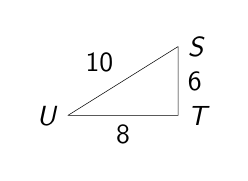
\begin{tikzpicture}[scale=0.7]
\tkzDefPoints{0/0/U, 2/0/T, 2/1.25/S}
\tkzDrawPolygon(T,U,S)
\tkzLabelPoints[left](U)
\tkzLabelPoints[right](T,S)
\tkzLabelSegment[below](U,T){8}
\tkzLabelSegment[right](S,T){6}
\tkzLabelSegment[above left](S,U){10}
\end{tikzpicture}
\hspace{0.1in}
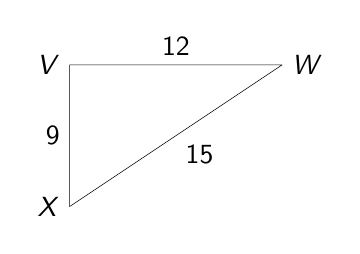
\begin{tikzpicture}[scale=0.9]
\tkzDefPoints{0/0/X, 3/2/W, 0/2/V}
\tkzDrawPolygon(V,W,X)
\tkzLabelPoints[left](X,V)
\tkzLabelPoints[right](W)
\tkzLabelSegment[left](V,X){9}
\tkzLabelSegment[above](V,W){12}
\tkzLabelSegment[below right](X,W){15}
\end{tikzpicture}
\end{minipage}
\begin{minipage}{0.4\textwidth}
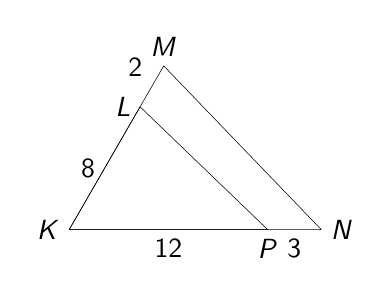
\begin{tikzpicture}[scale=0.8]
\tkzDefPoints{0/0/K, 4/0/N, 3.15/0/P}
\tkzDefShiftPoint[K](60:3){M}
\tkzDefShiftPoint[K](60:2.25){L}
\tkzDrawPolygon(K,M,N)
\tkzDrawPolygon(K,L,P)
\tkzLabelPoints[left](K,L)
\tkzLabelPoints[above](M)
\tkzLabelPoints[below](P)
\tkzLabelPoints[right](N)
\tkzLabelSegment[below](K,P){12}
\tkzLabelSegment[below](P,N){3}
\tkzLabelSegment[left](K,L){8}
\tkzLabelSegment[above left](L,M){2}
\end{tikzpicture}
\end{minipage}
\end{example}

\vfill 

\begin{example}
Find the value of $x$ in each. \newline 
\begin{multicols}{2}
\begin{enumerate}[(a)]
    \item \mbox{}  
    \item \mbox{} 
\end{enumerate}
\end{multicols}
\begin{minipage}{0.5\textwidth}
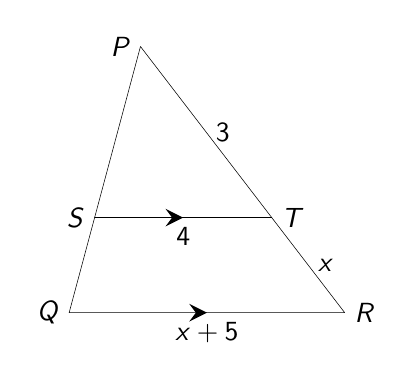
\begin{tikzpicture}[decoration={markings,
mark=at position 0.5 with {\arrow[scale=2]{>}};}]
\tkzDefPoints{0/0/Q, 3.5/0/R}
\tkzDefShiftPoint[Q](75:3.5){P}
\tkzDrawPolygon(P,Q,R)
\tkzDefShiftPoint[Q](75:1.25){S}
\tkzDefLine[parallel=through S](Q,R)
\tkzGetPoint{U}
%\tkzDrawSegment(S,U)
\tkzInterLL(S,U)(P,R)
\tkzGetPoint{T}
\tkzDrawSegment(S,T)
\tkzMarkSegments[mark=>](S,T Q,R)
\tkzLabelPoints[left](P,S,Q)
\tkzLabelPoints[right](T,R)
\tkzLabelSegment[below](Q,R){$x+5$}
\tkzLabelSegment[below](S,T){4}
\tkzLabelSegment[right](P,T){3}
\tkzLabelSegment[right](T,R){$x$}
\end{tikzpicture}
\end{minipage}
\begin{minipage}{0.4\textwidth}
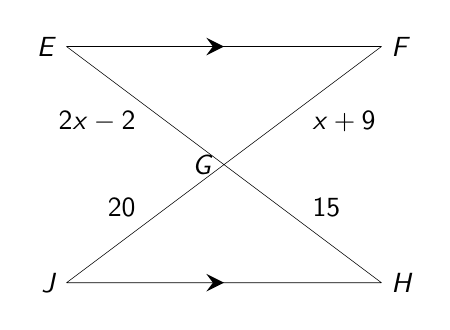
\begin{tikzpicture}[decoration={markings,
mark=at position 0.5 with {\arrow[scale=2]{>}};}]
\tkzDefPoints{0/0/J, 4/0/H, 0/3/E, 4/3/F}
\tkzDrawPolygon(J,H,E,F)
\tkzInterLL(F,J)(E,H)
\tkzGetPoint{G}
\tkzLabelPoints[left](E,G,J)
\tkzLabelPoints[right](F,H)
\tkzMarkSegments[mark=>](E,F J,H)
\tkzLabelSegment[left, yshift=0.2cm](J,G){20}
\tkzLabelSegment[left, yshift=-0.2cm](E,G){$2x-2$}
\tkzLabelSegment[right, yshift=0.2cm](G,H){15}
\tkzLabelSegment[right, yshift=-0.2cm](F,G){$x+9$}
\end{tikzpicture}
\end{minipage}
\end{example}

\vfill 

% \begin{example}
% Show that $\triangle ABC \sim \triangle DEF$ if
% \newline\\

% $A$(3, $-2$), $B(-1$, 0), C(4, 4)   \quad   $D$(7, $-5$), $E(-2.5$, 0), $F$(10, 10)
% \end{example}


\end{document}
